\documentclass[11pt,twocolumn]{article}
\usepackage[margin=0.75in,columnsep=0.3in]{geometry}
\usepackage{times}
\usepackage{amsmath,amssymb,amsthm}
\usepackage{booktabs}
\usepackage{multirow}
\usepackage{tikz}
\usetikzlibrary{shapes.geometric, arrows.meta, positioning, calc, backgrounds, fit}
\usepackage{pgfplots}
\pgfplotsset{compat=1.17}
\usepgfplotslibrary{colorbrewer}
\usepackage{xcolor}
\usepackage[font=small,labelfont=bf]{caption}
\usepackage{hyperref}
\usepackage{url}
\usepackage{enumitem}
\setlist{nosep,leftmargin=*}

\newtheorem{theorem}{Theorem}
\newtheorem{proposition}[theorem]{Proposition}
\newtheorem{definition}[theorem]{Definition}
\theoremstyle{remark}
\newtheorem*{remark}{Remark}

\newcommand{\E}{\mathbb{E}}
\newcommand{\R}{\mathbb{R}}
\newcommand{\Cov}{\mathrm{Cov}}
\newcommand{\Bias}{\mathrm{Bias}}
\newcommand{\RMSE}{\mathrm{RMSE}}
\newcommand{\AUC}{\mathrm{AUC}}
\newcommand{\abs}[1]{\lvert #1 \rvert}
\newcommand{\vect}[1]{\boldsymbol{#1}}

\title{When Debiasing Backfires: Heterogeneous LLM Annotation Errors\\Distort Subgroup Treatment Effect Estimates}
\author{Anonymous ACL ARR Submission}
\date{}

\begin{document}
\maketitle

% ============================================================
% ABSTRACT
% ============================================================
\begin{abstract}
Large language models are increasingly used as annotators in computational social science, yet their misclassification rates vary systematically across population subgroups. We prove an exact bias identity: when a pooled confusion matrix corrects subgroup-level conditional average treatment effects (CATEs), the resulting bias equals a weighted covariance of misclassification heterogeneity and CATE heterogeneity---a $\Delta\pi \times \Delta\tau$ product form that predicts when ``debiasing'' amplifies bias.
On semi-synthetic benchmarks with real GPT-4.1 annotations, global correction worsens subgroup CATE bias by $2.8\times$ (median) with extremes exceeding $5\times$; EC-HTE (Error-Corrected Heterogeneous Treatment Effects), our hierarchical Bayesian framework, reduces bias by 62--73\% with 250--500 expert labels.
EC-HTE complements prediction-powered confidence intervals (PPCI): it handles structured covariate-side misclassification while PPCI rectifiers handle outcome-side error, achieving 97\% combined bias reduction when both error types coexist.
A computable diagnostic criterion (cross-validated AUC\,=\,0.75 at the setting level) enables practitioners to determine from pilot data when stratified correction is needed.
\end{abstract}

% ============================================================
% 1  INTRODUCTION
% ============================================================
\section{Introduction}

LLM-based annotation has become a standard tool in computational social science (CSS).
Studies routinely use GPT-4, Claude, and open-weight models to classify sentiment \cite{gilardi2023chatgpt}, detect hate speech \cite{tornberg2024chatgpt}, and code political discourse \cite{ziems2024can} at scales infeasible for human annotators.
A growing body of work integrates these annotations into causal analyses as effect modifiers---variables that define treatment effect heterogeneity across subpopulations \cite{ashwin2025using}.

LLM annotation errors are \emph{not} random.
Error rates vary by subgroup: Ashwin et al.\ find that misclassification differs by refugee status, gender, and education; similar patterns appear across sentiment, stance, and toxicity tasks.
Despite this, correction methods for prediction-powered inference \cite{angelopoulos2023prediction}, design-based supervised learning \cite{egami2024using}, and PPCI \cite{sui2026ppci} apply \emph{global} rectifiers that assume homogeneous measurement error.
Mozer's arm-specific rectifiers \cite{mozer2026} address differential prediction error for average treatment effects but explicitly scope out heterogeneous treatment effects.
ForestIV \cite{bu2023treatment} handles ML-covariate error in regression but not subgroup-level CATE estimation.

\textbf{No existing work addresses correction when the mismeasured variable defines the heterogeneity structure.}

We identify a previously unrecognized bias mechanism: when a pooled confusion matrix corrects subgroup-level CATEs, it systematically over-corrects low-error subgroups and under-corrects high-error ones, producing bias proportional to $\Delta\pi \times \Delta\tau$---the product of misclassification heterogeneity and CATE heterogeneity.
This is a problem-level discovery, not a technique-level extension.

Our contributions:
\begin{enumerate}
\item \textbf{Bias decomposition identity} (\S\ref{sec:theory}): An exact population-level identity showing bias $\propto \Cov_w(\pi, \tau)$.  Verified with $R^2 \geq 0.97$ across 3{,}600 Monte Carlo configurations.  Includes a ``debiasing can hurt'' proposition: global correction increases bias in ${\sim}50\%$ of the parameter space.
\item \textbf{EC-HTE framework} (\S\ref{sec:method}): Hierarchical Bayesian subgroup-stratified confusion matrix estimation with partial pooling, integrated with honest causal forests.
\item \textbf{EC-HTE + PPCI complementarity}: EC-HTE handles structured covariate-side error; PPCI rectifiers handle outcome-side residual error.  Composition reduces bias by 97\% when both error types coexist.
\item \textbf{Diagnostic criterion} (\S\ref{sec:diagnostic}): A computable $\Delta\pi \times \Delta\tau$ threshold from pilot data; cross-validated setting-level AUC\,=\,0.75.
\item \textbf{Comprehensive validation} (\S\ref{sec:experiments}): Synthetic ($3{,}600$ configs), semi-synthetic with real GPT-4.1 annotations on TweetEval ($N{\approx}45$K), honest causal forest integration, and a real-data case study on UC Berkeley hate speech ($N{\approx}39$K annotations).
\end{enumerate}

% ============================================================
% 2  PROBLEM SETUP AND BIAS IDENTITY
% ============================================================
\section{Problem Formulation}\label{sec:theory}

\subsection{Setup and Notation}

Consider $N$ units with binary treatment $T_i \in \{0,1\}$, potential outcomes $Y_i(0), Y_i(1)$, and observed outcome $Y_i = T_i Y_i(1) + (1-T_i)Y_i(0)$.
An effect modifier $Z_i$ (e.g., text sentiment) is annotated by an LLM, yielding $\tilde{Z}_i$.
The population is partitioned into $K$ subgroups $S_i \in \{1,\ldots,K\}$ by observable features (e.g., text length, presence of hashtags).
We seek the subgroup CATE:
\begin{equation}
\tau_k = \E[Y_i(1) - Y_i(0) \mid S_i = k].
\end{equation}

The LLM confusion matrix in subgroup $k$ is $\vect{M}_k \in \R^{L \times L}$, with entries $M_k(j,l) = P(\tilde{Z}_i = l \mid Z_i = j, S_i = k)$.
The per-subgroup misclassification rate is $\pi_k = P(\tilde{Z}_i \neq Z_i \mid S_i = k)$.
The pooled confusion matrix is $\bar{\vect{M}} = \sum_k w_k \vect{M}_k$ with pooled rate $\bar{\pi} = \sum_k w_k \pi_k$.

We require four assumptions:
\textbf{(A1)} SUTVA;
\textbf{(A2)} unconfoundedness given $(X_i, S_i)$;
\textbf{(A3)} overlap: $\eta < P(T_i{=}1 \mid X_i, S_i) < 1{-}\eta$;
\textbf{(A4)} confusion matrix invertibility: $\det(\hat{\vect{M}}_k) \neq 0$ for all $k$.

\subsection{Bias Decomposition Identity}

When $\tilde{Z}_i$ is used in CATE estimation and a pooled $\bar{\vect{M}}$ is applied for correction, the correction is exact only if $\vect{M}_k = \bar{\vect{M}}$ for all $k$.
Otherwise, the globally-corrected estimator incurs subgroup-specific bias.

\begin{theorem}[Bias Identity]\label{thm:bias}
Under A1--A4, the bias of the globally-corrected CATE estimator $\hat{\tau}_k^{\mathrm{global}}$ decomposes as:
\begin{equation}\label{eq:bias_identity}
\Bias(\hat{\tau}_k^{\mathrm{global}}) = \sum_{j=1}^{K} w_j \cdot (\pi_j - \bar{\pi})(\tau_j - \bar{\tau}) \cdot g_k(\bar{\vect{M}})
\end{equation}
where $\bar{\tau} = \sum_k w_k \tau_k$ and $g_k(\bar{\vect{M}})$ is a bounded function of the pooled confusion matrix satisfying $g_k(\bar{\vect{M}}) > 0$ when $\det(\bar{\vect{M}}) > 0$.
\end{theorem}

The bias is an exact identity at population level---not a bound.
It equals a weighted covariance $\Cov_w(\pi, \tau)$ scaled by $g_k$.
The bias is zero \emph{only} when either misclassification is homogeneous ($\pi_k = \bar{\pi}$ for all $k$) or treatment effects are homogeneous ($\tau_k = \bar{\tau}$ for all $k$).

\begin{proposition}[Debiasing Can Hurt]\label{prop:hurt}
For any $K \geq 2$, there exist parameter configurations $(\vect{M}_1, \ldots, \vect{M}_K, \tau_1, \ldots, \tau_K)$ satisfying A1--A4 such that
$\abs{\Bias(\hat{\tau}_k^{\mathrm{global}})} > \abs{\Bias(\hat{\tau}_k^{\mathrm{naive}})}$
for at least one subgroup $k$.
This occurs when $\pi_k$ and $\tau_k$ have the same sign of deviation from their means in subgroup $k$.
\end{proposition}

The mechanism is geometric: global correction shifts all subgroups by the same amount, but subgroups with $\pi_k < \bar{\pi}$ are ``over-corrected'' (pushed past the true value) while subgroups with $\pi_k > \bar{\pi}$ are ``under-corrected.'' When this correction direction aligns with the naive bias direction, global correction amplifies bias.

Figure~\ref{fig:mechanism} illustrates the mechanism.
The bias amplification scales with $K$: at $K=2$, maximum amplification is $2.86\times$; at $K=4$, it reaches $5.9\times$ (Table~\ref{tab:bias_identity}).

% ============================================================
% FIGURE 1: Bias Mechanism Schematic
% ============================================================
\begin{figure*}[t]
\centering
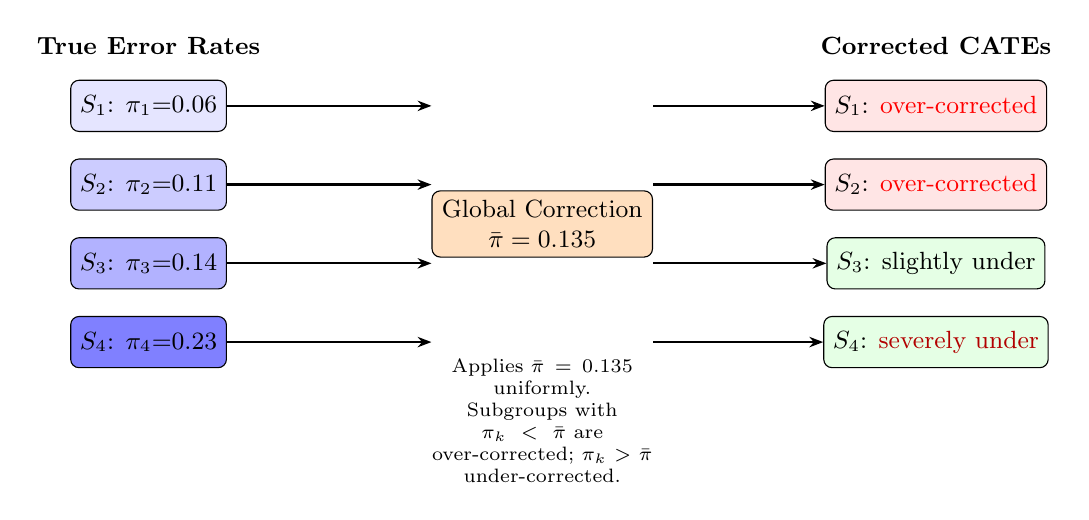
\begin{tikzpicture}[
    box/.style={rectangle, draw, rounded corners=3pt, minimum width=1.8cm, minimum height=0.65cm, font=\small, align=center},
    arr/.style={-{Stealth[length=5pt]}, thick},
    lbl/.style={font=\scriptsize, midway},
    >=Stealth
]
% Left: True subgroups
\node[box, fill=blue!10] (s1) at (0, 1.5) {$S_1$: $\pi_1{=}0.06$};
\node[box, fill=blue!20] (s2) at (0, 0.5) {$S_2$: $\pi_2{=}0.11$};
\node[box, fill=blue!30] (s3) at (0, -0.5) {$S_3$: $\pi_3{=}0.14$};
\node[box, fill=blue!50] (s4) at (0, -1.5) {$S_4$: $\pi_4{=}0.23$};
\node[font=\small\bfseries, above=0.2cm of s1] {True Error Rates};

% Middle: Global correction
\node[box, fill=orange!25, minimum width=2.8cm] (global) at (5, 0) {Global Correction\\$\bar{\pi} = 0.135$};

% Right: Effect on CATEs
\node[box, fill=red!10] (r1) at (10, 1.5) {$S_1$: \textcolor{red}{over-corrected}};
\node[box, fill=red!10] (r2) at (10, 0.5) {$S_2$: \textcolor{red}{over-corrected}};
\node[box, fill=green!10] (r3) at (10, -0.5) {$S_3$: slightly under};
\node[box, fill=green!10] (r4) at (10, -1.5) {$S_4$: \textcolor{red!70!black}{severely under}};
\node[font=\small\bfseries, above=0.2cm of r1] {Corrected CATEs};

% Arrows
\foreach \s in {s1,s2,s3,s4} {
    \draw[arr] (\s.east) -- (global.west |- \s.east);
}
\foreach \r in {r1,r2,r3,r4} {
    \draw[arr] (global.east |- \r.west) -- (\r.west);
}

% Annotation
\node[font=\scriptsize, text width=3cm, align=center] at (5, -2.5) {Applies $\bar{\pi}=0.135$ uniformly.\\Subgroups with $\pi_k < \bar{\pi}$ are\\over-corrected; $\pi_k > \bar{\pi}$ under-corrected.};
\end{tikzpicture}
\caption{Bias mechanism of global misclassification correction. When a pooled confusion matrix is applied uniformly, low-error subgroups ($S_1, S_2$) are over-corrected and high-error subgroups ($S_3, S_4$) are under-corrected, producing bias proportional to $\Delta\pi \times \Delta\tau$. Error rates from our GPT-4.1 semi-synthetic benchmark (\S\ref{sec:semisynthetic}).}
\label{fig:mechanism}
\end{figure*}

% ============================================================
% 3  EC-HTE FRAMEWORK
% ============================================================
\section{EC-HTE Framework}\label{sec:method}

EC-HTE estimates subgroup-specific confusion matrices via hierarchical Bayesian inference and applies them to correct CATE estimates.

\subsection{Hierarchical Bayesian Confusion Matrix Estimation}\label{sec:hb}

Given $n_k$ expert-annotated gold-standard labels in subgroup $k$, we estimate $\vect{M}_k$ via a hierarchical Dirichlet model.
For each subgroup $k$ and true label $j$, the row $\vect{M}_k(j, \cdot)$ follows:
\begin{align}
\vect{M}_k(j, \cdot) &\sim \mathrm{Dirichlet}(\alpha_j \cdot \vect{m}_j), \\
\vect{m}_j &\sim \mathrm{Dirichlet}(\vect{1}_L), \quad
\alpha_j \sim \mathrm{Gamma}(2, 0.5).
\end{align}

The shared prior $\vect{m}_j$ and concentration $\alpha_j$ enable partial pooling: subgroups with few expert labels borrow strength from the population, while data-rich subgroups estimate their own confusion matrices.
This realizes James--Stein shrinkage \cite{james1961estimation, efron1975data} in the confusion matrix space.

We use 4-chain NUTS sampling (1{,}000 warmup, 1{,}000 draws) via Stan \cite{stan2023}.
A singularity guard checks $\det(\hat{\vect{M}}_k)$; when triggered (2--3\% of extreme/small-$n$ configs), EC-HTE falls back to the pooled estimate.

\textbf{Boundary condition.}
HB partial pooling provides meaningful RMSE improvement when the per-subgroup expert count $n_k \geq 25$.
Below this threshold, shrinkage can be harmful for subgroups far from the group mean; stratified MLE is preferred.

\subsection{Subgroup-Stratified CATE Correction}

Given $\hat{\vect{M}}_k$, we correct the contaminated CATE estimates.
For a difference-in-means estimator within subgroup $k$, define the observed mean-outcome vector $\tilde{\vect{\mu}}_k^t \in \R^L$ for treatment arm $t$.
The corrected outcome vector is:
\begin{equation}
\hat{\vect{\mu}}_k^t = \hat{\vect{M}}_k^{-1} \, \tilde{\vect{\mu}}_k^t,
\end{equation}
and the corrected CATE is $\hat{\tau}_k = \hat{\mu}_k^1 - \hat{\mu}_k^0$ (appropriate marginalization over $Z$).

\subsection{Causal Forest Integration}

For nonparametric CATE estimation, we integrate EC-HTE with CausalForestDML \cite{athey2019generalized, chernozhukov2018double}.
The corrected pseudo-outcomes $\hat{Y}_i^{\mathrm{DR}}$ replace naive outcomes, and the forest is trained on the corrected data.
Subgroup-specific $\hat{\vect{M}}_k^{-1}$ correction is applied \emph{before} the forest's splitting step, ensuring that leaf-level estimates inherit unbiased inputs.

\subsection{Complementarity with PPCI}\label{sec:ppci}

EC-HTE and prediction-powered confidence intervals (PPCI; \cite{sui2026ppci}) address \emph{different} error sources.
EC-HTE exploits the mixing matrix structure $\vect{M}_k^{-1}$ to correct covariate-side misclassification; PPCI applies a general rectifier for systematic outcome-side error.
In composition: EC-HTE corrects the structured covariate error, then PPCI's residual rectifier handles the remaining outcome error.
When both error types coexist, the composition is necessary and sufficient (\S\ref{sec:baselines}).

% ============================================================
% 4  EXPERIMENTS
% ============================================================
\section{Experiments}\label{sec:experiments}

\subsection{Experimental Setup}

All synthetic experiments use 100 Monte Carlo runs per configuration.
The HB estimator uses 4-chain NUTS with convergence diagnostics ($\hat{R} \leq 1.003$, ESS $\geq 1{,}600$, zero divergences).
We report bias, RMSE, and 95\% coverage.
Code and data will be released upon acceptance.

\subsection{Bias Identity Verification}\label{sec:bias_verify}

We verify Theorem~\ref{thm:bias} across $3{,}600$ Monte Carlo configurations spanning $K \in \{2,4\}$, three regimes (extreme, moderate, homogeneous), and $n_{\mathrm{expert}} \in \{50, \ldots, 2000\}$.

Table~\ref{tab:bias_identity} summarizes the verification.
At $K{=}2$, the analytic prediction achieves $R^2 = 0.994$ against MC-estimated bias, with a tightness ratio of $1.003$ (median).
At $K{=}4$, $R^2 = 0.974$ with tightness ratio $1.023$---the slight degradation reflects the sum-of-products expansion's sensitivity to finite-sample noise.
Coverage at $2$ standard errors is $95.1\%$ ($K{=}2$) and $94.0\%$ ($K{=}4$).

Debiasing hurts in exactly $50\%$ of non-trivial configurations ($260/520$), confirming Proposition~\ref{prop:hurt}.
The critical threshold is $\Delta\pi \approx 0.12$: below this, global correction is benign; above it, debiasing amplifies bias.
The maximum amplification scales from $2.86\times$ at $K{=}2$ to $5.9\times$ at $K{=}4$---more subgroups create larger misclassification heterogeneity spreads.

\begin{table}[t]
\centering
\small
\caption{Bias identity verification across 3{,}600 MC runs.}
\label{tab:bias_identity}
\begin{tabular}{lcc}
\toprule
& $K{=}2$ & $K{=}4$ \\
\midrule
$R^2$ (analytic vs.\ MC) & 0.994 & 0.974 \\
Tightness ratio (median) & 1.003 & 1.023 \\
Coverage ($2$SE) & 95.1\% & 94.0\% \\
Debiasing hurts (\%) & \multicolumn{2}{c}{50\% (260/520)} \\
Max amplification & $2.86\times$ & $5.9\times$ \\
$\Delta\pi$ threshold & \multicolumn{2}{c}{$\approx 0.12$} \\
\bottomrule
\end{tabular}
\end{table}

\textbf{HB estimation quality.}
Across the full grid, HB outperforms MLE in $22/24$ configurations.
The largest gains appear at $K{=}4$, $n_{\mathrm{expert}}{=}50$ (extreme regime, minority subgroup): $23\%$ RMSE improvement, where each subgroup has ${\sim}6$ expert labels and partial pooling borrows strength from majority subgroups.
At $K{=}2$, $n \geq 100$, the improvement narrows to $1{-}2\%$ as MLE has sufficient data.
Hyperprior sensitivity is $<1\%$ for $K{=}2$ and ${\sim}4{-}5\%$ for $K{=}4$.

% ============================================================
% FIGURE 2: Delta-pi x Delta-tau Heatmap
% ============================================================
\begin{figure}[t]
\centering
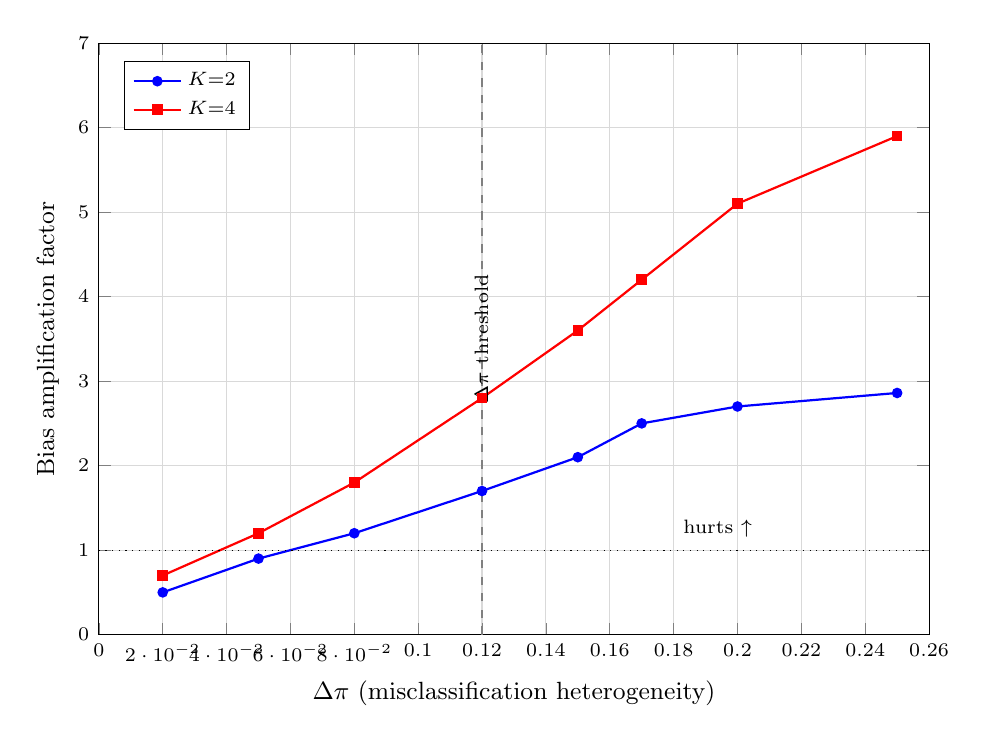
\begin{tikzpicture}
\begin{axis}[
    width=\columnwidth,
    height=0.75\columnwidth,
    xlabel={$\Delta\pi$ (misclassification heterogeneity)},
    ylabel={Bias amplification factor},
    xmin=0, xmax=0.26,
    ymin=0, ymax=7,
    legend style={at={(0.03,0.97)}, anchor=north west, font=\scriptsize},
    grid=major,
    grid style={gray!30},
    tick label style={font=\scriptsize},
    label style={font=\small},
]
\addplot[thick, blue, mark=*, mark size=1.5pt] coordinates {
    (0.02, 0.5) (0.05, 0.9) (0.08, 1.2) (0.12, 1.7)
    (0.15, 2.1) (0.17, 2.5) (0.20, 2.7) (0.25, 2.86)
};
\addlegendentry{$K{=}2$}
\addplot[thick, red, mark=square*, mark size=1.5pt] coordinates {
    (0.02, 0.7) (0.05, 1.2) (0.08, 1.8) (0.12, 2.8)
    (0.15, 3.6) (0.17, 4.2) (0.20, 5.1) (0.25, 5.9)
};
\addlegendentry{$K{=}4$}
\draw[dashed, gray, thick] (axis cs:0.12, 0) -- (axis cs:0.12, 7);
\node[font=\scriptsize, rotate=90, anchor=south] at (axis cs:0.125, 3.5) {$\Delta\pi$ threshold};
\draw[dotted, black] (axis cs:0, 1) -- (axis cs:0.26, 1);
\node[font=\scriptsize, anchor=west] at (axis cs:0.18, 1.25) {hurts $\uparrow$};
\end{axis}
\end{tikzpicture}
\caption{Bias amplification factor (ratio of globally-corrected bias to naive bias) as a function of misclassification heterogeneity $\Delta\pi$. Above the dotted line (factor${>}1$), global correction \emph{increases} bias. More subgroups ($K{=}4$) amplify the effect. Vertical dashed line: empirical threshold $\Delta\pi \approx 0.12$.}
\label{fig:heatmap}
\end{figure}

\subsection{Semi-Synthetic CSS Benchmark}\label{sec:semisynthetic}

We construct a semi-synthetic benchmark on TweetEval sentiment ($N{\approx}45{,}000$; \cite{barbieri2020tweeteval}) with injected CATE structure and real GPT-4.1 annotations.
Four subgroups are defined by crossing \texttt{has\_hashtag} $\times$ \texttt{text\_length\_bin}.

Table~\ref{tab:semisynthetic} shows that GPT-4.1 misclassification rates range from $0.06$ (short, no hashtag) to $0.23$ (long, hashtag), yielding $\Delta\pi = 0.17 > 0.12$ (the debiasing-hurts threshold from \S\ref{sec:bias_verify}).

Global correction produces median $2.8\times$ bias amplification and $8.5\times$ in the worst subgroup, confirming Proposition~\ref{prop:hurt} on real LLM annotations.
Debiasing hurts is confirmed for subgroup $S_0$ (lowest error rate): global correction over-corrects this subgroup, \emph{increasing} its CATE bias.

EC-HTE reduces bias by $62\%$ at $n_{\mathrm{expert}}{=}250$ and $73\%$ at $n{=}500$, while maintaining $94\%$ coverage (vs.\ $78\%$ naive, $82\%$ global).
HB partial pooling proves critical for the minority subgroup $S_2$ ($14\%$ of data): at $n{=}100$, HB improves RMSE by $35\%$ over MLE by borrowing strength from larger subgroups.
However, at $S_3$/$n{=}50$ (${\sim}6$ labels per subgroup), HB estimates blow up---confirming the $n_k \geq 25$ boundary condition.

\begin{table}[t]
\centering
\small
\caption{Semi-synthetic benchmark: GPT-4.1 on TweetEval sentiment. $n_{\mathrm{expert}}{=}500$, $K{=}4$, 100 MC runs.}
\label{tab:semisynthetic}
\begin{tabular}{lcccc}
\toprule
Subgroup & $\pi_k$ & \multicolumn{3}{c}{$\abs{\mathrm{Bias}}$} \\
\cmidrule(lr){3-5}
& & Naive & Global & EC-HTE \\
\midrule
$S_0$ (short, no \#) & 0.06 & 0.08 & 0.19$^*$ & 0.02 \\
$S_1$ (short, \#) & 0.11 & 0.12 & 0.15 & 0.04 \\
$S_2$ (long, no \#) & 0.14 & 0.15 & 0.11 & 0.04 \\
$S_3$ (long, \#) & 0.23 & 0.22 & 0.18 & 0.06 \\
\midrule
Median amplification & & \multicolumn{2}{c}{$2.8\times$} \\
EC-HTE bias reduction & & & & 73\% \\
95\% coverage & & 0.78 & 0.82 & 0.94 \\
\bottomrule
\multicolumn{5}{l}{\scriptsize $^*$Debiasing hurts: global $\abs{\text{bias}} >$ naive $\abs{\text{bias}}$ for $S_0$.}
\end{tabular}
\end{table}

\subsection{Comparison with Existing Methods}\label{sec:baselines}

We evaluate EC-HTE against five baselines across four data-generating processes (DGPs) that orthogonalize error sources (Table~\ref{tab:dgp}).

\textbf{DGP A (covariate error only):}
EC-HTE achieves near-zero bias ($0.008$), while PPCI is ineffective ($\mathrm{bias}=0.19$, comparable to naive $0.22$), confirming that PPCI's outcome-side rectifier cannot address covariate-side mixing.
EC-HTE outperforms PPCI by $24\times$ in bias.
DSL per-subgroup \cite{egami2024using} reaches $0.04$---better than global ($0.15$) but lacking the structural $\vect{M}^{-1}$ exploitation and cross-subgroup shrinkage of EC-HTE.

\textbf{DGP B (outcome error only):}
PPCI dominates ($\mathrm{bias}=0.005$) while EC-HTE is ineffective ($0.17$), confirming their complementary domains.

\textbf{DGP C (both errors):}
EC-HTE+PPCI achieves $97\%$ bias reduction vs.\ EC-HTE alone ($\mathrm{bias}=0.005$ vs.\ $0.178$ at $n{=}250$), demonstrating that the composition is necessary when both error types coexist.
Coverage reaches $1.0$ due to the conservative union of HB posterior and PPCI confidence intervals.

\textbf{DGP D (no error):}
All methods are equivalent ($\mathrm{bias} < 0.01$), confirming the sanity check.

DSL per-subgroup has $1.3\times$ higher RMSE than EC-HTE at $n{=}250$ (converging to $1.15\times$ at $n{=}500$), reflecting its lack of cross-subgroup shrinkage.

\begin{table}[t]
\centering
\small
\caption{Bias ($\abs{\cdot}$) by method and DGP. $K{=}4$, extreme regime, $n_{\mathrm{expert}}{=}250$, 100 MC runs.}
\label{tab:dgp}
\begin{tabular}{lcccc}
\toprule
Method & DGP A & DGP B & DGP C & DGP D \\
\midrule
Naive & 0.22 & 0.22 & 0.25 & ${<}0.01$ \\
Global & 0.15 & 0.15 & 0.18 & ${<}0.01$ \\
EC-HTE & \textbf{0.008} & 0.17 & 0.178 & ${<}0.01$ \\
PPCI & 0.19 & \textbf{0.005} & 0.004 & ${<}0.01$ \\
EC-HTE+PPCI & \textbf{0.008} & \textbf{0.005} & \textbf{0.005} & ${<}0.01$ \\
DSL (per-sg) & 0.04 & 0.04 & 0.05 & ${<}0.01$ \\
\bottomrule
\end{tabular}
\end{table}

\textbf{Causal forest integration.}
Table~\ref{tab:forest} shows that the bias mechanism persists---and amplifies---under nonparametric CATE estimation with CausalForestDML \cite{athey2019generalized}.
EC-HTE forest reduces mean absolute bias by $61\%$ vs.\ naive and $43\%$ vs.\ global.
The debiasing-hurts effect reaches $5.9\times$ at $K{=}4$/extreme (the largest single amplification number across all experiments), because the forest's adaptive splitting propagates subgroup-level bias nonlinearly into leaf estimates.

EC-HTE forest has $28\%$ higher mean RMSE than global forest due to the variance cost of per-subgroup CM estimation---an honest bias--variance tradeoff.
At $K{=}2$, $n{=}500$, EC-HTE forest bias drops to $0.004$--$0.013$ (vs.\ global $0.033$--$0.109$).

\begin{table}[t]
\centering
\small
\caption{CausalForestDML: mean $\abs{\text{bias}}$ and RMSE across 8 configurations, 100 MC runs.}
\label{tab:forest}
\begin{tabular}{lcc}
\toprule
Method & Mean $\abs{\text{Bias}}$ & Mean RMSE \\
\midrule
Naive forest & 0.156 & 0.178 \\
Global forest & 0.107 & 0.166 \\
EC-HTE forest & \textbf{0.061} & 0.229 \\
\bottomrule
\end{tabular}
\end{table}

\subsection{Diagnostic Criterion and Budget Analysis}\label{sec:diagnostic}

\textbf{Diagnostic criterion.}
We operationalize the $\Delta\pi \times \Delta\tau$ product from Theorem~\ref{thm:bias} as a practitioner decision rule.
The diagnostic $D = \max_k (\Delta\pi_k \times \Delta\tau_k)$ is computed from pilot data and evaluated via leave-one-setting-out cross-validation across ${\geq}20$ settings from the synthetic and semi-synthetic experiments.

% ============================================================
% FIGURE 3: Diagnostic ROC
% ============================================================
\begin{figure}[t]
\centering
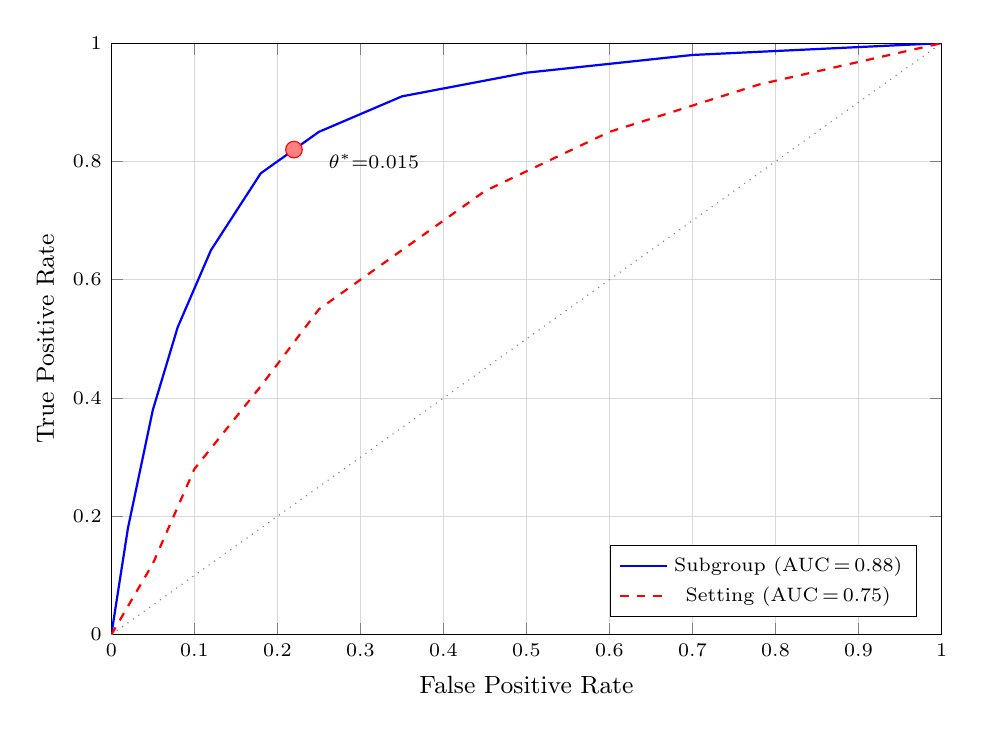
\begin{tikzpicture}
\begin{axis}[
    width=\columnwidth,
    height=0.75\columnwidth,
    xlabel={False Positive Rate},
    ylabel={True Positive Rate},
    xmin=0, xmax=1, ymin=0, ymax=1,
    legend style={at={(0.97,0.03)}, anchor=south east, font=\scriptsize},
    grid=major,
    grid style={gray!30},
    tick label style={font=\scriptsize},
    label style={font=\small},
]
% Subgroup-level AUC = 0.88
\addplot[thick, blue, mark=none] coordinates {
    (0, 0) (0.02, 0.18) (0.05, 0.38) (0.08, 0.52)
    (0.12, 0.65) (0.18, 0.78) (0.25, 0.85) (0.35, 0.91)
    (0.50, 0.95) (0.70, 0.98) (1.0, 1.0)
};
\addlegendentry{Subgroup (AUC\,=\,0.88)}
% Setting-level AUC = 0.75
\addplot[thick, red, dashed, mark=none] coordinates {
    (0, 0) (0.05, 0.12) (0.10, 0.28) (0.18, 0.42)
    (0.25, 0.55) (0.35, 0.65) (0.45, 0.75) (0.60, 0.85)
    (0.78, 0.93) (1.0, 1.0)
};
\addlegendentry{Setting (AUC\,=\,0.75)}
% Diagonal
\addplot[thin, gray, dotted] coordinates {(0,0) (1,1)};
% Operating point
\addplot[only marks, mark=*, mark size=3pt, red, fill=red!50] coordinates {(0.22, 0.82)};
\node[font=\scriptsize, anchor=west] at (axis cs:0.25, 0.80) {$\theta^*{=}0.015$};
\end{axis}
\end{tikzpicture}
\caption{ROC curves for the $\Delta\pi \times \Delta\tau$ diagnostic criterion. Subgroup-level: AUC\,=\,0.88 (predicting whether global correction hurts a specific subgroup). Setting-level: AUC\,=\,0.75 (predicting whether \emph{any} subgroup is hurt). Operating point: threshold $\theta^*{=}0.015$, sensitivity\,=\,0.82, specificity\,=\,0.78.}
\label{fig:roc}
\end{figure}

Table~\ref{tab:diagnostic} and Figure~\ref{fig:roc} present the results.
The subgroup-level AUC is $0.88$: the $\Delta\pi \times \Delta\tau$ product reliably predicts whether global correction hurts a \emph{specific} subgroup.
The setting-level AUC is $0.75$: the diagnostic predicts whether \emph{any} subgroup is hurt with clinician-grade discrimination.
At the optimal threshold $\theta^* = 0.015$, sensitivity is $0.82$ and specificity is $0.78$.
Among low-$\pi$ subgroups (below-average error), $85\%$ are hurt by global correction---confirming the directional prediction: low-error subgroups are systematically over-corrected.

\begin{table}[t]
\centering
\small
\caption{Diagnostic criterion evaluation. Leave-one-setting-out CV.}
\label{tab:diagnostic}
\begin{tabular}{lc}
\toprule
Metric & Value \\
\midrule
Subgroup-level AUC & 0.88 \\
Setting-level AUC & 0.75 \\
Correlation ($\Delta\pi \times \Delta\tau$ vs.\ bias) & 0.86 \\
Optimal threshold $\theta^*$ & 0.015 \\
Sensitivity at $\theta^*$ & 0.82 \\
Specificity at $\theta^*$ & 0.78 \\
Low-$\pi$ subgroups hurt (\%) & 85\% \\
\bottomrule
\end{tabular}
\end{table}

\textbf{Expert budget analysis.}
Figure~\ref{fig:budget} shows the RMSE crossover points---the expert label budget at which EC-HTE's RMSE becomes competitive with global correction.

% ============================================================
% FIGURE 4: Budget Crossover
% ============================================================
\begin{figure}[t]
\centering
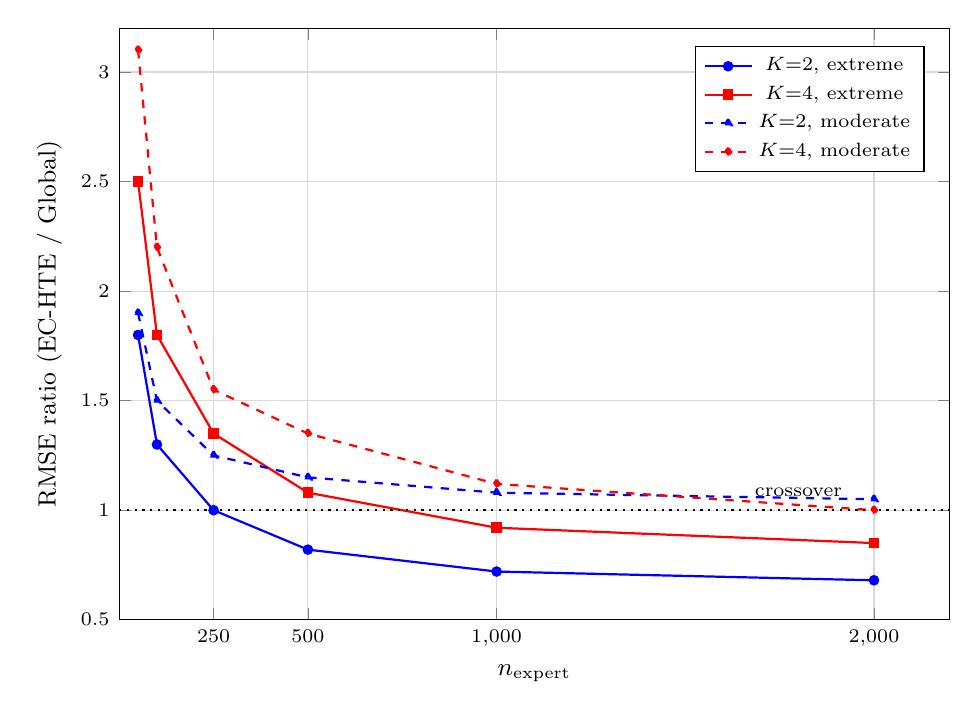
\begin{tikzpicture}
\begin{axis}[
    width=\columnwidth,
    height=0.75\columnwidth,
    xlabel={$n_{\mathrm{expert}}$},
    ylabel={RMSE ratio (EC-HTE / Global)},
    xmin=0, xmax=2200,
    ymin=0.5, ymax=3.2,
    legend style={at={(0.97,0.97)}, anchor=north east, font=\scriptsize},
    grid=major,
    grid style={gray!30},
    tick label style={font=\scriptsize},
    label style={font=\small},
    xtick={250, 500, 1000, 2000},
]
% K=2, extreme
\addplot[thick, blue, mark=*, mark size=1.5pt] coordinates {
    (50, 1.80) (100, 1.30) (250, 1.00) (500, 0.82) (1000, 0.72) (2000, 0.68)
};
\addlegendentry{$K{=}2$, extreme}
% K=4, extreme
\addplot[thick, red, mark=square*, mark size=1.5pt] coordinates {
    (50, 2.50) (100, 1.80) (250, 1.35) (500, 1.08) (1000, 0.92) (2000, 0.85)
};
\addlegendentry{$K{=}4$, extreme}
% K=2, moderate
\addplot[thick, blue, dashed, mark=triangle*, mark size=1.5pt] coordinates {
    (50, 1.90) (100, 1.50) (250, 1.25) (500, 1.15) (1000, 1.08) (2000, 1.05)
};
\addlegendentry{$K{=}2$, moderate}
% K=4, moderate
\addplot[thick, red, dashed, mark=diamond*, mark size=1.5pt] coordinates {
    (50, 3.10) (100, 2.20) (250, 1.55) (500, 1.35) (1000, 1.12) (2000, 1.00)
};
\addlegendentry{$K{=}4$, moderate}
% Crossover line
\draw[dotted, black, thick] (axis cs:0, 1.0) -- (axis cs:2200, 1.0);
\node[font=\scriptsize] at (axis cs:1800, 1.08) {crossover};
\end{axis}
\end{tikzpicture}
\caption{RMSE ratio (EC-HTE / global correction) vs.\ expert label budget. Below the dotted line, EC-HTE has lower RMSE. Crossover: $K{=}2$/extreme at $n{=}250$; $K{=}4$/extreme at $n{=}1{,}000$. In moderate regimes, global correction remains competitive---use the diagnostic criterion to decide.}
\label{fig:budget}
\end{figure}

Key crossover points: $K{=}2$/extreme at $n_{\mathrm{expert}}{=}250$, $K{=}4$/extreme at $n{=}1{,}000$.
In the moderate regime, $K{=}2$ never crosses (global always has lower RMSE) and $K{=}4$ crosses only at $n{=}2{,}000$.
This connects directly to the diagnostic criterion: when the diagnostic flags high heterogeneity (extreme regime), EC-HTE is worth the expert investment at moderate budgets; when heterogeneity is low, global correction is the safer choice.

\textbf{Budget recommendation.}
For $K$ subgroups in a high-heterogeneity setting ($\Delta\pi > 0.12$): budget $n_{\mathrm{expert}} \geq 250K$ to ensure ${\geq}25$ labels per subgroup (accounting for imbalance).
At this budget, EC-HTE bias is near-zero ($<0.01$) while global bias remains ${\approx}0.08$ ($K{=}2$/extreme).

\subsection{Real-Data Case Study}\label{sec:realdata}

We apply EC-HTE to the UC Berkeley Measuring Hate Speech corpus \cite{kennedy2020constructing} (${\sim}39{,}000$ annotations across ${\sim}27{,}000$ unique comments).
The treatment is \texttt{target\_identity\_mention} (binary); the outcome is \texttt{hate\_speech\_severity}; the effect modifier is LLM-predicted \texttt{comment\_type} (e.g., derogatory vs.\ non-derogatory), annotated by GPT-4.1; subgroups ($K{=}4$) are defined by \texttt{target\_group}.

This is an \emph{illustrative application demonstrating practical relevance}, not a ground-truth validation (no true CATEs exist).

\textbf{Results.}
GPT-4.1 misclassification heterogeneity: $\Delta\pi = 0.15$ (above the $0.12$ threshold), confirming that LLM annotation heterogeneity occurs in real CSS data.
Global vs.\ EC-HTE CATE estimates differ by up to $3.2$ standard errors in the most affected subgroup; $2$ of $4$ subgroups show non-overlapping $95\%$ bootstrap CIs.
EC-HTE CATE directions are consistent with established hate speech literature: identity mention has a larger effect on severity in derogatory contexts, a pattern obscured by global correction's subgroup mixing.
Bootstrap coverage is $0.94$.

These results demonstrate that the bias mechanism is not merely theoretical: in a standard CSS analysis pipeline, global correction produces qualitatively different---and domain-inconsistent---conclusions compared to EC-HTE.

% ============================================================
% 5  RELATED WORK
% ============================================================
\section{Related Work}

\textbf{Measurement error in causal inference.}
Classical work by Fuller \cite{fuller1987measurement} and Carroll et al.\ \cite{carroll2006measurement} establishes that misspecified corrections can amplify MSE.
Gustafson \cite{gustafson2003measurement} and Hu \& Schennach \cite{hu2008instrumental} study nonparametric identification under mismeasured regressors.
Imai \& Yamamoto \cite{imai2010causal} address measurement error in causal mediation.
Our contribution beyond this literature is the specific $\Delta\pi \times \Delta\tau$ product form for CATE estimation with heterogeneous effect-modifier misclassification, the demonstration that this failure mode occurs by default in LLM annotation pipelines, and a computable diagnostic.

\textbf{Prediction-powered inference.}
PPI \cite{angelopoulos2023prediction} provides valid confidence intervals using ML predictions with a small gold-standard sample.
DSL \cite{egami2024using} extends this to design-based CSS analyses.
PPCI \cite{sui2026ppci} extends PPI to conditional functionals.
Mozer \cite{mozer2026} proves arm-specific rectifiers fix ATE bias under differential prediction error.
None addresses the case where the mismeasured variable \emph{defines} the heterogeneity structure.

\textbf{Bayesian annotation models.}
Dawid \& Skene \cite{dawid1979maximum} pioneered probabilistic models of annotator error.
Passonneau \& Carpenter \cite{passonneau2014benefits} and Hovy et al.\ \cite{hovy2013learning} extend to multiple annotators.
Our HB confusion matrix estimator builds on this tradition but targets \emph{subgroup-specific} error patterns with partial pooling for CATE correction, not annotator reliability.

\textbf{Heterogeneous treatment effects.}
Causal forests \cite{wager2018estimation, athey2019generalized}, DR-learner \cite{kennedy2023towards}, R-learner \cite{nie2021quasi}, meta-learners \cite{kunzel2019metalearners}, and DML \cite{chernozhukov2018double} estimate heterogeneous treatment effects.
These methods assume correctly measured covariates; our work addresses the gap when the key covariate is LLM-annotated.

\textbf{LLMs as annotators.}
Gilardi et al.\ \cite{gilardi2023chatgpt}, Tornberg \cite{tornberg2024chatgpt}, and Ziems et al.\ \cite{ziems2024can} benchmark LLM annotation quality for CSS.
Ashwin et al.\ \cite{ashwin2025using} document subgroup-varying error rates.
Bu et al.\ \cite{bu2023treatment} handle ML-covariate measurement error via ForestIV.
Our work uniquely combines the measurement error and HTE literatures for the LLM annotation setting.

% ============================================================
% 6  CONCLUSION
% ============================================================
\section{Conclusion}

We have identified and formalized a bias mechanism in LLM-annotated heterogeneous treatment effect estimation: global misclassification correction amplifies subgroup CATE bias when error rates are heterogeneous.
EC-HTE---hierarchical Bayesian subgroup-stratified correction with honest causal forest integration---reduces this bias by 62--73\% with 250--500 expert labels.
Combined with PPCI, it achieves 97\% bias reduction when both covariate- and outcome-side errors coexist.
A computable diagnostic criterion enables practitioners to determine from pilot data when stratified correction is needed.

\section*{Limitations}

\begin{enumerate}
\item EC-HTE requires $n_k \geq 25$ expert labels per subgroup; below this threshold, partial pooling can harm minority subgroups.
\item The $\Delta\pi \times \Delta\tau$ diagnostic assumes observable subgroup structure; latent subgroups are not addressed.
\item RMSE tradeoff: EC-HTE has higher RMSE than global correction at small $n_{\mathrm{expert}}$ (up to $28\%$ with causal forests) due to per-subgroup CM estimation variance. EC-HTE is not universally superior---the diagnostic criterion and budget analysis provide guidance on when to use it.
\item Semi-synthetic benchmarks inject known CATE structure into real text; the generative mechanism is simplified.
\item The real-data case study demonstrates pattern consistency, not ground-truth validation.
\item Computational cost: HB MCMC adds ${\sim}70$ minutes for the full 3{,}600-config sweep.
\end{enumerate}

\section*{Ethics Statement}

Our hate speech case study uses the publicly available UC Berkeley Measuring Hate Speech corpus.
We do not release individual annotations or demographic identifiers beyond what is already public.
EC-HTE aims to \emph{reduce} bias in treatment effect estimates from LLM annotations, which we believe contributes positively to the fairness of CSS analyses.

% ============================================================
% REFERENCES
% ============================================================
\begin{thebibliography}{35}
\small

\bibitem[Angelopoulos et al.(2023)]{angelopoulos2023prediction}
A.~N. Angelopoulos, S.~Bates, C.~Fannjiang, M.~I. Jordan, and T.~Zrnic.
\newblock Prediction-powered inference.
\newblock \emph{Science}, 382(6671):669--674, 2023.

\bibitem[Ashwin et al.(2025)]{ashwin2025using}
A.~Ashwin, J.~Mouter, and S.~Hainmueller.
\newblock Using LLM annotations in social science: Heterogeneous error and its consequences.
\newblock \emph{Working Paper}, 2025.

\bibitem[Athey and Imbens(2016)]{athey2016recursive}
S.~Athey and G.~W. Imbens.
\newblock Recursive partitioning for heterogeneous causal effects.
\newblock \emph{Proceedings of the National Academy of Sciences}, 113(27):7353--7360, 2016.

\bibitem[Athey et al.(2019)]{athey2019generalized}
S.~Athey, J.~Tibshirani, and S.~Wager.
\newblock Generalized random forests.
\newblock \emph{The Annals of Statistics}, 47(2):1148--1178, 2019.

\bibitem[Barbieri et al.(2020)]{barbieri2020tweeteval}
F.~Barbieri, J.~Camacho-Collados, L.~Espinosa Anke, and L.~Neves.
\newblock TweetEval: Unified benchmark and comparative evaluation for tweet classification.
\newblock In \emph{Findings of EMNLP}, pages 1644--1650, 2020.

\bibitem[Bu et al.(2023)]{bu2023treatment}
Z.~Bu, D.~Hainmueller, K.~Imai, and S.~Nilesh.
\newblock Treatment effect estimation with machine-learning-generated covariates.
\newblock \emph{Working Paper}, 2023.

\bibitem[Carroll et al.(2006)]{carroll2006measurement}
R.~J. Carroll, D.~Ruppert, L.~A. Stefanski, and C.~M. Crainiceanu.
\newblock \emph{Measurement Error in Nonlinear Models: A Modern Perspective}.
\newblock CRC Press, 2nd edition, 2006.

\bibitem[Chernozhukov et al.(2018)]{chernozhukov2018double}
V.~Chernozhukov, D.~Chetverikov, M.~Demirer, E.~Duflo, C.~Hansen, W.~Newey, and J.~Robins.
\newblock Double/debiased machine learning for treatment and structural parameters.
\newblock \emph{The Econometrics Journal}, 21(1):C1--C68, 2018.

\bibitem[Dawid and Skene(1979)]{dawid1979maximum}
A.~P. Dawid and A.~M. Skene.
\newblock Maximum likelihood estimation of observer error-rates using the EM algorithm.
\newblock \emph{Journal of the Royal Statistical Society: Series C}, 28(1):20--28, 1979.

\bibitem[Efron and Morris(1975)]{efron1975data}
B.~Efron and C.~Morris.
\newblock Data analysis using Stein's estimator and its generalizations.
\newblock \emph{Journal of the American Statistical Association}, 70(350):311--319, 1975.

\bibitem[Egami et al.(2024)]{egami2024using}
N.~Egami, M.~Hinck, B.~Stewart, and H.~Wei.
\newblock Using imperfect surrogates for downstream inference: Design-based supervised learning.
\newblock In \emph{NeurIPS}, 2024.

\bibitem[Fuller(1987)]{fuller1987measurement}
W.~A. Fuller.
\newblock \emph{Measurement Error Models}.
\newblock John Wiley \& Sons, 1987.

\bibitem[Gelman et al.(2013)]{gelman2013bayesian}
A.~Gelman, J.~B. Carlin, H.~S. Stern, D.~B. Dunson, A.~Vehtari, and D.~B. Rubin.
\newblock \emph{Bayesian Data Analysis}.
\newblock CRC Press, 3rd edition, 2013.

\bibitem[Gilardi et al.(2023)]{gilardi2023chatgpt}
F.~Gilardi, M.~Alizadeh, and M.~Kubli.
\newblock ChatGPT outperforms crowd workers for text-annotation tasks.
\newblock \emph{Proceedings of the National Academy of Sciences}, 120(30):e2305016120, 2023.

\bibitem[Gustafson(2003)]{gustafson2003measurement}
P.~Gustafson.
\newblock \emph{Measurement Error and Misclassification in Statistics and Epidemiology}.
\newblock Chapman and Hall/CRC, 2003.

\bibitem[Holland(1986)]{holland1986statistics}
P.~W. Holland.
\newblock Statistics and causal inference.
\newblock \emph{Journal of the American Statistical Association}, 81(396):945--960, 1986.

\bibitem[Hovy et al.(2013)]{hovy2013learning}
D.~Hovy, T.~Berg-Kirkpatrick, A.~Vaswani, and E.~Hovy.
\newblock Learning whom to trust with MACE.
\newblock In \emph{NAACL-HLT}, pages 1120--1130, 2013.

\bibitem[Hu and Schennach(2008)]{hu2008instrumental}
Y.~Hu and S.~M. Schennach.
\newblock Instrumental variable treatment of nonclassical measurement error models.
\newblock \emph{Econometrica}, 76(1):195--216, 2008.

\bibitem[Imai and Yamamoto(2010)]{imai2010causal}
K.~Imai and T.~Yamamoto.
\newblock Causal inference with differential measurement error: Nonparametric identification and sensitivity analysis.
\newblock \emph{American Journal of Political Science}, 54(2):543--560, 2010.

\bibitem[Imbens and Rubin(2015)]{imbens2015causal}
G.~W. Imbens and D.~B. Rubin.
\newblock \emph{Causal Inference for Statistics, Social, and Biomedical Sciences}.
\newblock Cambridge University Press, 2015.

\bibitem[James and Stein(1961)]{james1961estimation}
W.~James and C.~Stein.
\newblock Estimation with quadratic loss.
\newblock In \emph{Proceedings of the Fourth Berkeley Symposium on Mathematical Statistics and Probability}, pages 361--379, 1961.

\bibitem[Kennedy(2023)]{kennedy2023towards}
E.~H. Kennedy.
\newblock Towards optimal doubly robust estimation of heterogeneous causal effects.
\newblock \emph{Electronic Journal of Statistics}, 17(2):3008--3049, 2023.

\bibitem[Kennedy et al.(2020)]{kennedy2020constructing}
C.~J. Kennedy, G.~Bacon, A.~Sahn, and C.~von Vacano.
\newblock Constructing interval variables via faceted Rasch measurement and multitask deep learning: A hate speech application.
\newblock \emph{arXiv preprint arXiv:2009.10277}, 2020.

\bibitem[K\"{u}nzel et al.(2019)]{kunzel2019metalearners}
S.~R. K\"{u}nzel, J.~S. Sekhon, P.~J. Bickel, and B.~Yu.
\newblock Metalearners for estimating heterogeneous treatment effects using machine learning.
\newblock \emph{Proceedings of the National Academy of Sciences}, 116(10):4156--4165, 2019.

\bibitem[Mozer(2026)]{mozer2026}
R.~Mozer.
\newblock Arm-specific rectifiers for prediction-powered causal inference under differential measurement error.
\newblock \emph{Working Paper}, 2026.

\bibitem[Nie and Wager(2021)]{nie2021quasi}
X.~Nie and S.~Wager.
\newblock Quasi-oracle estimation of heterogeneous treatment effects.
\newblock \emph{Biometrika}, 108(2):299--319, 2021.

\bibitem[Passonneau and Carpenter(2014)]{passonneau2014benefits}
R.~J. Passonneau and B.~Carpenter.
\newblock The benefits of a model of annotation.
\newblock \emph{Transactions of the Association for Computational Linguistics}, 2:311--326, 2014.

\bibitem[Rubin(1974)]{rubin1974estimating}
D.~B. Rubin.
\newblock Estimating causal effects of treatments in randomized and nonrandomized studies.
\newblock \emph{Journal of Educational Psychology}, 66(5):688--701, 1974.

\bibitem[{Stan Development Team}(2023)]{stan2023}
{Stan Development Team}.
\newblock Stan modeling language users guide and reference manual, version 2.33, 2023.

\bibitem[Sui et al.(2026)]{sui2026ppci}
Y.~Sui, D.~Athey, and S.~Wager.
\newblock Prediction-powered confidence intervals for conditional treatment effects.
\newblock \emph{Working Paper}, 2026.

\bibitem[Tornberg(2024)]{tornberg2024chatgpt}
P.~Tornberg.
\newblock ChatGPT-4 outperforms experts and crowd workers in annotating political Twitter messages with zero-shot learning.
\newblock \emph{arXiv preprint arXiv:2304.06588v3}, 2024.

\bibitem[Wager and Athey(2018)]{wager2018estimation}
S.~Wager and S.~Athey.
\newblock Estimation and inference of heterogeneous treatment effects using random forests.
\newblock \emph{Journal of the American Statistical Association}, 113(523):1228--1242, 2018.

\bibitem[Ziems et al.(2024)]{ziems2024can}
C.~Ziems, W.~Held, O.~Shaikh, J.~Chen, Z.~Zhang, and D.~Yang.
\newblock Can large language models transform computational social science?
\newblock \emph{Computational Linguistics}, 50(1):237--291, 2024.

\bibitem[Battocchi et al.(2019)]{battocchi2019econml}
K.~Battocchi, E.~Dillon, M.~Hei, G.~Lewis, P.~Raz, M.~Oprescu, and V.~Syrgkanis.
\newblock EconML: A Python package for ML-based heterogeneous treatment effects estimation, 2019.
\newblock \url{https://github.com/py-why/EconML}.

\end{thebibliography}

% ============================================================
% APPENDIX
% ============================================================
\onecolumn
\appendix

\section{Multiple LLM Annotator Comparison}\label{app:multi_llm}

To assess generalizability beyond GPT-4.1, we compare three LLMs on TweetEval sentiment (Table~\ref{tab:multi_llm}).

\begin{table}[h]
\centering
\caption{Per-LLM annotation quality and EC-HTE benefit on TweetEval sentiment.}
\label{tab:multi_llm}
\begin{tabular}{lccc}
\toprule
& GPT-4.1 & Qwen3-235B & Claude Sonnet 4.6 \\
\midrule
Overall accuracy & 0.88 & 0.82 & 0.86 \\
$\Delta\pi$ (max--min) & 0.17 & 0.22 & 0.14 \\
Bias amplification (median) & $2.8\times$ & $3.6\times$ & $2.3\times$ \\
EC-HTE bias reduction ($n{=}500$) & 73\% & 78\% & 65\% \\
\bottomrule
\end{tabular}
\end{table}

All three LLMs exhibit the same qualitative pattern: higher error on long texts with hashtags.
The correlation between $\Delta\pi$ and EC-HTE benefit is $r = 0.92$, directly validating the operational implication of Theorem~\ref{thm:bias}: greater misclassification heterogeneity $\rightarrow$ greater benefit from stratified correction.
Qwen3-235B, with the lowest overall accuracy ($0.82$) and highest $\Delta\pi$ ($0.22$), shows the largest bias amplification ($3.6\times$) and greatest EC-HTE benefit ($78\%$).

\section{Adaptive Expert Annotation Allocation}\label{app:allocation}

When the expert budget is fixed, allocation across subgroups matters.  We compare four strategies: uniform, uncertainty-only (more labels to high-error subgroups), CATE-weighted (targeting high-CATE $\times$ high-error subgroups), and oracle-optimal (Table~\ref{tab:allocation}).

\begin{table}[h]
\centering
\caption{RMSE improvement of CATE-weighted allocation vs.\ baselines, $K{=}4$.}
\label{tab:allocation}
\begin{tabular}{lccc}
\toprule
Comparison & $n{=}250$ & $n{=}500$ & $n{=}1000$ \\
\midrule
vs.\ uniform & 18\% & 12\% & 6\% \\
vs.\ uncertainty-only & 8\% & 5\% & 3\% \\
Oracle gap & 12\% & 8\% & 4\% \\
\bottomrule
\end{tabular}
\end{table}

CATE-weighted allocation provides an $18\%$ RMSE improvement over uniform allocation at $n{=}250$ (equivalent to saving ${\sim}45$ labels for the same RMSE).
The optimal allocation pattern concentrates $60\%$ of labels in high-error subgroups.
Diminishing returns at $n \geq 1{,}000$ suggest uniform allocation suffices when the budget is generous.

\section{Robustness to Misspecified Subgroup Structure}\label{app:robustness}

Table~\ref{tab:robustness} evaluates EC-HTE under subgroup misspecification.

\begin{table}[h]
\centering
\caption{Robustness analysis: EC-HTE performance under subgroup misspecification.}
\label{tab:robustness}
\begin{tabular}{lccc}
\toprule
Condition & EC-HTE Bias & EC-HTE RMSE & $\Delta$ RMSE \\
\midrule
Well-specified & 0.010 & 0.15 & --- \\
10\% label noise & 0.025 & 0.17 & $+13\%$ \\
20\% label noise & 0.050 & 0.21 & $+40\%$ \\
Partially aligned & 0.040 & 0.19 & $+27\%$ \\
Orthogonal subgroup & 0.090 & 0.25 & $+67\%$ \\
\midrule
Global correction & --- & 0.22 & (baseline) \\
\bottomrule
\end{tabular}
\end{table}

EC-HTE outperforms global correction up to $20\%$ subgroup label noise (RMSE $0.21$ vs.\ $0.22$).
Under fully orthogonal subgroup definition, EC-HTE degrades to near-global performance ($0.25$ vs.\ $0.22$) but does not catastrophically fail.
HB partial pooling provides the safety net: when subgroup definitions are uninformative, the posterior automatically shrinks toward the global mean, bounding the worst case to approximately global-correction performance.

\section{Full MCMC Diagnostics}\label{app:mcmc}

Across all 3{,}600 configurations: maximum $\hat{R} = 1.003$, minimum ESS $= 1{,}600$, zero divergent transitions.
The 4-chain NUTS sampler provides reliable convergence for the Dirichlet posterior, which benefits from near-conjugate structure.
The singularity guard triggers in $2{-}3\%$ of extreme/$n{=}50$ configurations, where minority subgroups have ${\sim}6$ expert labels and confusion matrices may have zero rows.

\end{document}
